\section{Design Overview}\label{sec:overview}

VeLoc leverages both the floor map of the parking structure and inertial data of the driver's smartphone to track the vehicle's location. As shown in Figure~\ref{pix:overview}, Veloc consists of the following three components.
\begin{enumerate}
  \item \textbf{Pose estimation} estimates the pose, the relative orientation of the smartphone's three axes to those of the vehicle. This information is needed to transform the inertial data sensed along the phone's axes into those of the vehicle. Then the inertial data is also used to detect whether the vehicle is moving or stationary (described in Section~\ref{sec:pose}).
  \item \textbf{Landmark detection algorithms} detect three types of ground features common to parking structures, namely speed bumps, turns and slopes. These are used as calibration points so uncertainties in the vehicle's location can be greatly reduced once a landmark is detected (Section~\ref{sec:landmark}).
  \item \textbf{Realtime tracking} module employs an augmented particle filter based method to estimate the states of a vehicle (including its location, orientation, and velocity) using a probabilistic model. It exploits the constraints from detected landmarks and the floor map to reduce the uncertainty in the states so that the vehicle's location can be determined(Section~\ref{sec:tracking}).
\end{enumerate}
\begin{figure}[h]
  \centering
  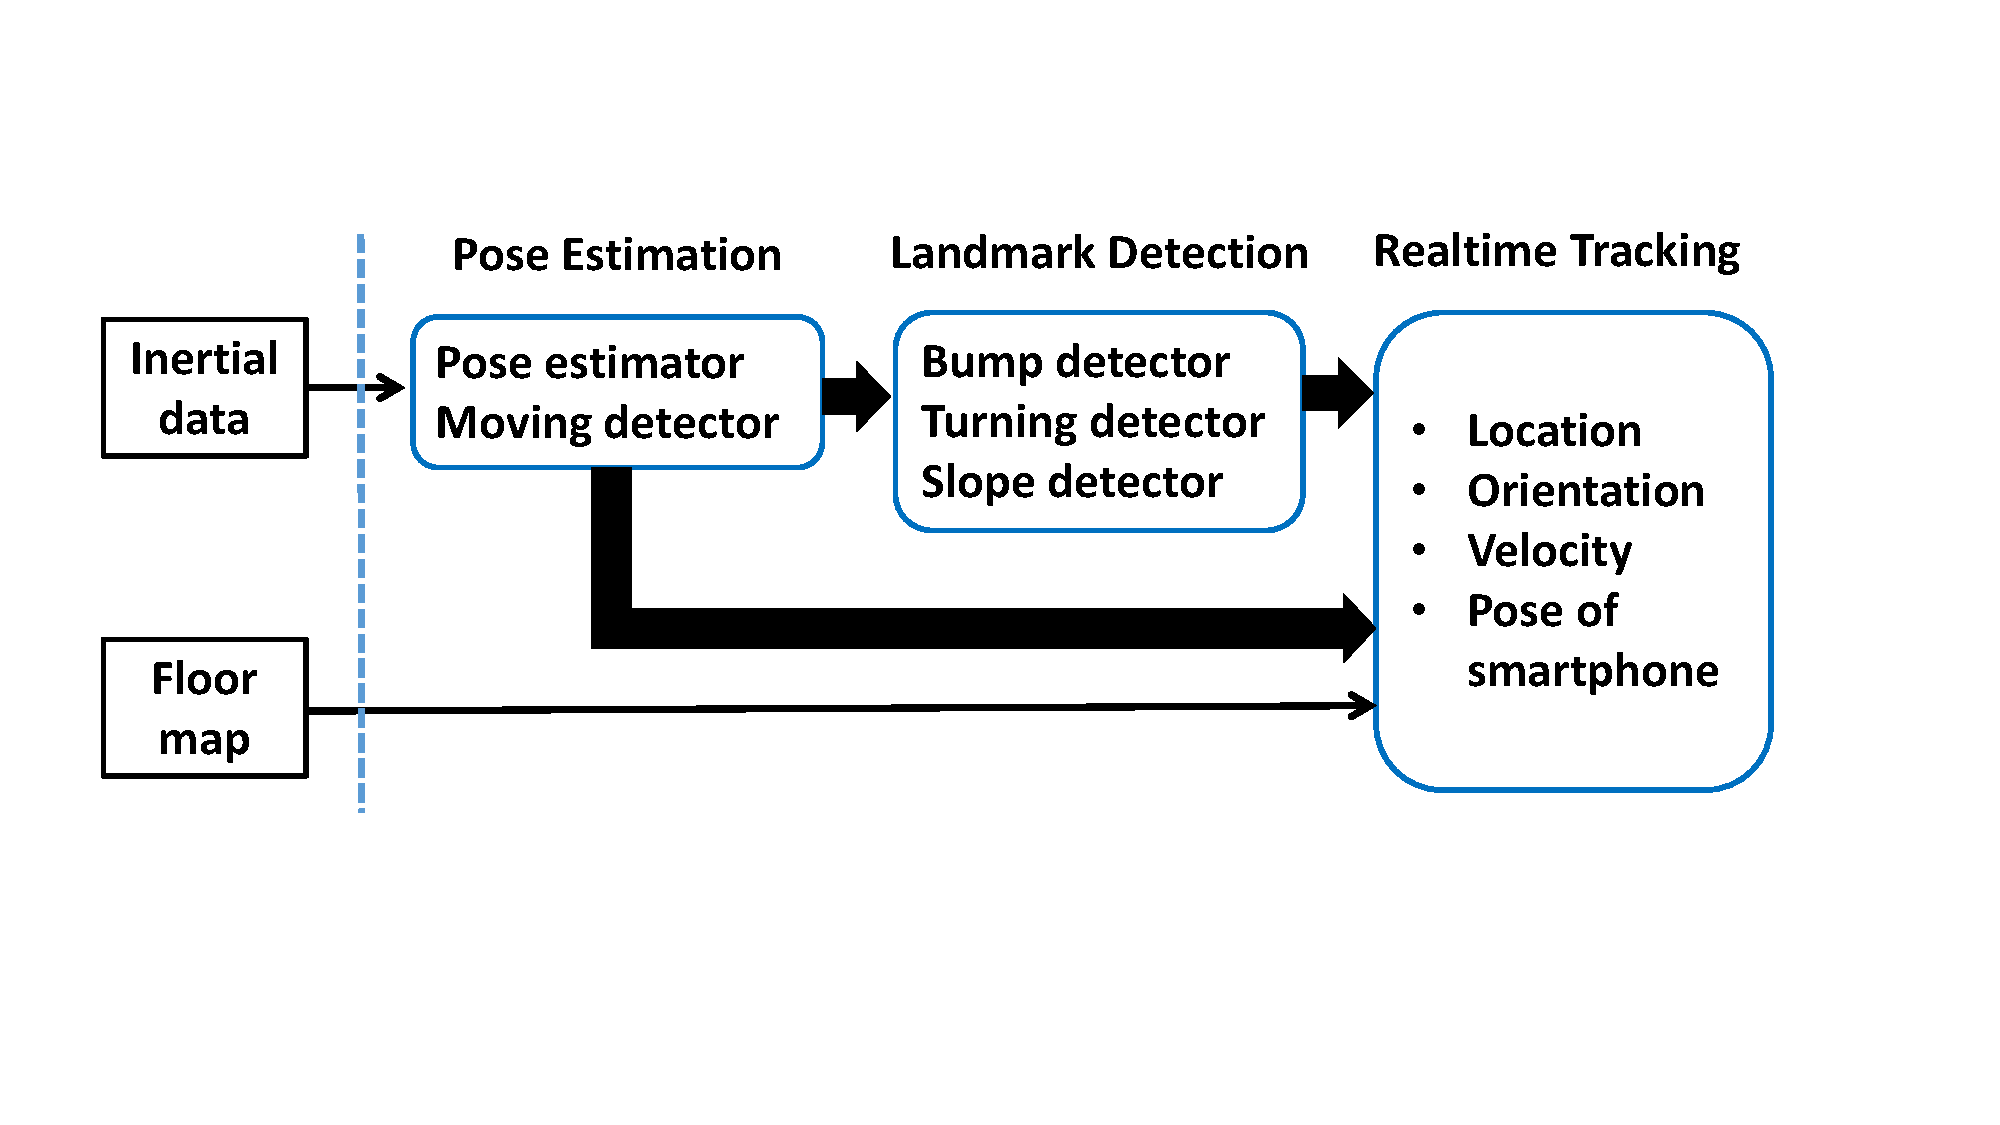
\includegraphics[width=0.5\textwidth]{overview}\\
  \caption{Three components of VeLoc. Inertial data is used to compute the smartphone's pose in the vehicle, then it is further processed to detect certain landmarks during driving, and the augmented particle filter harnesses constraints from landmark detection and the floor map for vehicle localization.}\label{pix:overview}
\end{figure}

